%!TEX root = Tesi.tex

\section{Progettazione sniffer}
Il primo passo per lo sviluppo è stato prendere confidenza sia con l'ambiente di lavoro che con il dispositivo della RedBear. Testare un semplice progetto, come il lampeggio di un led, si è comunque rivelata un'operazione non banale.
L'SDK che la Nordic fornisce contiene esempi modificati appositamente per le sue board di sviluppo, come la PCA10040 o la PCA10056, descritte nel capitolo \ref{nordic_board}, che come già accennato hanno una piedinatura e una dotazione di periferiche differente rispetto al nano2. Il primo passo è stato quindi quello di utilizzare una board supportata e modificarne la piedinatura delle periferiche connesse; il numero di led è stato ridotto a 1 solo connesso al pin 11 e sono stati rimossi i riferimenti a pulsanti connessi, perché non presenti sulla nostra periferica. \'E stato necessario modificare anche i collegamenti dei 4 pin relativi alla comunicazione UART come segue:
\begin{itemize}
\item[-] CTS pin 28
\item[-] RTS pin 2
\item[-] TX pin 29
\item[-] RX pin 30
\end{itemize}
Tutte queste modifiche sono state apportate al file pca10040.h che si trova nell'sdk nella cartella /components/boards .

Eseguendo una nuova compilazione e provando a scrivere il file .hex generato continuava a non funzionare. Dopo varie prove si è capito che mancavano delle librerie da cui il progetto dipendeva; esse sono contenute nel SOFTDEVICE, un file .hex che viene fornito già compilato nell'SDK, nella cartella /components/softdevice/s132/hex. Per tutti i progetti creati si usa la versione s132 del softdevice che è la più completa e contiene tutte le librerie necessarie per far funzionare il nano2 sia come dispositivo di tipo central che peripheral.

\subsection{UART}
Per visualizzare i dati intercettati via etere è necessario poter comunicare informazioni ad un dispositivo dotato di output video; nel nostro caso è stato utilizzato un PC, che avendo una gran capacità di memorizzazione può contenere tutti i dati catturati, per essere visualizzati ed analizzati anche in un secondo momento. Per trasferire questi dati abbiamo utilizzato una funzionalità supportata dal nano2, la trasmissione usando UART. \'E l'acronimo di Universal Asynchronous Receiver Transmitter, ovvero ricevitore trasmettitore asincrono/seriale, è un dispositivo hardware che converte flussi da un formato parallelo, tipicamente quelli usati all'interno di un processore, in formato seriale asincrono.
Inviare dati tramire UART è un'operazione che richiede pochi settaggi e quindi poche righe di codice, utilizzando le apposite funzioni di libreria messe a disposizione nella SDK. 

\begin{samepage}
All'interno di un progetto, va prima inizializzato il modulo fornendo le impostazioni che desideriamo usare:
\begin{itemize}
\item[-] Baudrate: il numero di simboli che vengono trasmessi in un secondo, determina la velocità di trasmissione.
\item[-] Control Flow: indica se utilizzare o meno le due linee aggiuntive destinate alla comunicazione UART ovvero, CTS (Clear To Send) e RTS (Ready To Send) per gestire lo scambio di dati, utile per annullare i conflitti trasmissivi.
\end{itemize}
Normalmente i settaggi sono inseriti nella funzione \emph{uart\_init()} che viene eseguita all'avvio del dispositivo.
\end{samepage}

Vanno inseriti dei caratteri di controllo per differenziare la fine di un pacchetto con l'inizio del successivo, ed eventualmente indicare informazioni aggiuntive al solo pacchetto, come la lunghezza dello stesso. \'E quindi stato inserito il carattere denominato MARKER del valore di 0xE0 all'inizio di ogni dato inserito; i 2 Byte successivi indicano la lunghezza dell'intero pacchetto, quindi comprendono anche i caratteri di controllo. Il quarto Byte viene usato per indicare il canale il cui è stato catturato il pacchetto e dal 5° Byte in poi si avrà ciò che è stato catturato, così come viene rilevato dal Nano2.
\begin{figure}[H]
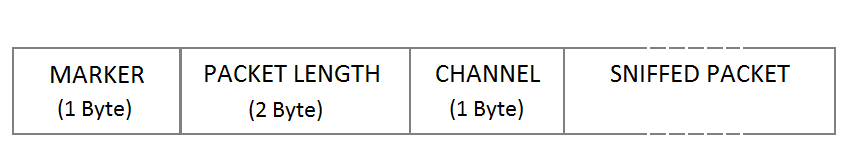
\includegraphics[width=320pt]{uart_packet}
\centering
\caption{Pacchetto inviato tramite UART che contiene il pacchetto sniffato e i campi di controllo.}
\end{figure}
Nel caso in cui all'interno del pacchetto stesso ci siano Byte del valore di 0xE0, che hanno lo stesso valore del Marker, per evitare di confonderli si raddoppia il Byte. In questo modo se nel pacchetto ricevuto si incontrerà un Byte singolo del valore del Marker, allora quello sarà un vero Marker che indica l'inizio di una nuova trasmissione; negli altri casi sarà un Byte del pacchetto, si dovrà quindi scartare il Byte successivo, che non fa parte dei dati catturati dallo Sniffer.

\subsection{NRF RADIO}
Il cuore del progetto, ovvero l'intercettazione dei pacchetti, viene creato utilizzando la struttura NRF\_ RADIO, che contiene tutti i possibili campi settabili per far funzionare il dispositivo Radio, contenuto all'interno del SoC nRF52832, nelle modalità che si desiderano.
\begin{figure}[H]
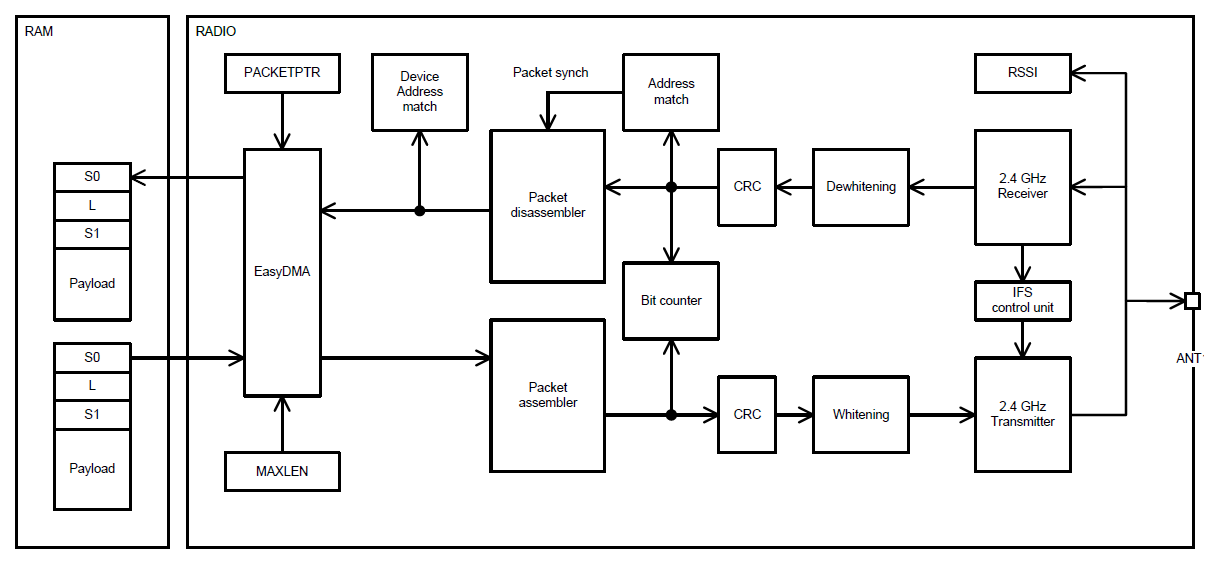
\includegraphics[width=400pt]{radio_block_diagram}
\centering
\caption{Diagramma a Blocchi del trasmettitore radio.}
\end{figure}
Il dispositivo Radio contiene un ricevitore e trasmettitore a 2.4 GHz, un assemblatore e disassemblatore di pacchetti automatico, un generatore e verificatore di CRC automatico che permettono in modo facile e veloce di ottenere il pacchetto ascoltato partendo da ciò che è stato ricevuto via radio. Include inoltre un Device Address Match, utile per quelle funzionalità che richiedono il filtraggio dei pacchetti in automatico, per ricevere solo quelli destinati o provenienti da un determinato indirizzo. Si è dimostrato molto utile anche il sistema RSSI\footnote{Received Signal Strength Indicator}, ovvero un sistema che calcola l'intensità del segnale ricevuto, per essere eventualmente filtrato se troppo lontano o debole.
In ogni ambiente in cui si è andato ad attivare lo sniffer erano sempre presenti nell'etere pacchetti di altri dispositivi che andavano a sommarsi ai dispositivi usati per il test, rendendo più difficile l'individuazione a video dei pacchetti di interesse; tramite la ricezione della potenza del segnale è stato possibile escludere dall'invio e quindi dalla visualizzazione tutti quei pacchetti dei dispositivi lontani dallo sniffer, quindi di non interesse, garantendo la visualizzazione dei soli pacchetti provenienti dai dispositivi sotto test.
Il sistema Radio integrato nel SoC della Nordic è pensato per essere utilizzato con più protocolli trasmissivi, oltre al Bluetooth Low Energy; vanno quindi indicati, in fase di configurazione la lunghezza in Byte delle varie parti di un pacchetto BLE, con particolare specifica del campo Length del pacchetto. I campi di cui andare a settare la grandezza sono SO, LENGTH ed S1.
Tramite il valore di PCNF0 della struttura NRF\_ RADIO è possibile configurare la lunghezza dei campi suddetti.



\begin{minted}[fontsize=\footnotesize]{c}
NRF_RADIO->PCNF0 = (
	(((1UL) <<RADIO_PCNF0_S0LEN_Pos)& RADIO_PCNF0_S0LEN_Msk) |  
	(((2UL) <<RADIO_PCNF0_S1LEN_Pos)& RADIO_PCNF0_S1LEN_Msk) |  
	(((6UL) <<RADIO_PCNF0_LFLEN_Pos)& RADIO_PCNF0_LFLEN_Msk)   
);
\end{minted}

Dove la lunghezza di S0 è espressa in Byte e contiene il primo Byte dell'header, dove sono contenute le informazioni sul tipo di pacchetto e sul tipo degli eventuali indirizzi contenuti nel Payload (pubblici o privati.
La lunghezza di S1 è espressa invece in bit; nel nostro caso è uguale a 2 perché per i pacchetti di tipo advertise nel secondo Byte dell'header 2 bit sono RFU e attribuiti quindi a questo campo:
La lunghezza del campo length è espressa sempre in bit, 6 nel nostro caso e contiene appunto la lunghezza in Byte del payload.

Il valore del campo PCNF1 configura altri parametri, come la lunghezza massima che può assumere il Payload, eventuali Byte di espansione di quest'ultimo, lunghezza dell'indirizzo, il tipo di endian da utilizzare (introdotto nel capitolo \ref{endian_bit}) 

\begin{minted}[fontsize=\footnotesize,breaklines]{c}
NRF_RADIO->PCNF1 = (
	(((37UL) << RADIO_PCNF1_MAXLEN_Pos) & RADIO_PCNF1_MAXLEN_Msk)  |                     
	(((0UL) << RADIO_PCNF1_STATLEN_Pos) & RADIO_PCNF1_STATLEN_Msk) |                     
	(((3UL) << RADIO_PCNF1_BALEN_Pos) & RADIO_PCNF1_BALEN_Msk)     |                     
	(((RADIO_PCNF1_ENDIAN_Little) << RADIO_PCNF1_ENDIAN_Pos&RADIO_PCNF1_ENDIAN_Msk) | 
	(((1UL) << RADIO_PCNF1_WHITEEN_Pos) & RADIO_PCNF1_WHITEEN_Msk)                        
);
\end{minted}

Da configurare all'interno della struttura NRF\_ RADIO è anche il canale in cui essere in ascolto; esso influenza 2 campi:
\begin{minted}[fontsize=\footnotesize,breaklines]{c}
NRF_RADIO->FREQUENCY = frequency_resolver(); 
NRF_RADIO->DATAWHITEIV = channel;
\end{minted}

FREQUENCY è il campo in cui scrivere la frequenza di ascolto, indicata a scarti di 2 MHz e con prima frequenza utile il valore 0, ha quindi un campo di escursione da 0 a 80 MHz. Viene calcolata tramite la funzione \emph{frequency\_resolver()} che si basa sull'indice del canale desiderato.
DTAWHITEIV va settato semplicemente con l'indice del canale e serve per inizializzare l'algoritmo che andrà a rimuovere il whitening dai pacchetti ricevuti.

Tramite l'Access Address e il CRCInit che vengono forniti alla Radio si riceveranno solo i pacchetti che corrispondono a questi valori. Per i pacchetti di Advertising l'Access Address è fisso e vale 0x8E89BED6. Esso all'interno della struttura Radio è diviso in 2 parti: il PREFIX0 e BASE0; per impostare la Radio per la ricezione dei pacchetti advertise, l'indirizzo va diviso come segue:

\begin{minted}[fontsize=\footnotesize,breaklines]{c}
NRF_RADIO->PREFIX0 = 0x8e;
NRF_RADIO->BASE0 = 0x89bed600; 
\end{minted}
Per i pacchetti di una connessione l'AA varia, ed è deciso dal device Central al momento della connessione ed inviato al device Peripheral nella CONNECT\_ REQ.

I parametri da impostare per quanto riguarda la gestione del CRC sono il CRCCNF che indica il numero di Byte di lunghezza del CRC, il CRCINIT che per i pacchetti di Advertise ha un valore fisso a 0x555555 ma che per una connessione varia in accordo con il valore contenuto nella CONNECT\_ REQ, ed il CRCPOLY, che per tutte le trasmissioni BLE è fisso al valore 0x65B.

\begin{minted}[fontsize=\footnotesize,breaklines]{c}
NRF_RADIO->CRCCNF  = (RADIO_CRCCNF_LEN_Three << RADIO_CRCCNF_LEN_Pos) |
            (RADIO_CRCCNF_SKIPADDR_Skip << RADIO_CRCCNF_SKIPADDR_Pos); 
NRF_RADIO->CRCINIT = 0x555555;  
NRF_RADIO->CRCPOLY = 0x00065B;
\end{minted}

Dopo aver correttamente impostato la Radio è possibile mettere in ascolto il dispositivo per la ricezione dei pacchetti. la ricezione viene descritta ed attuata tramite una macchina a stati; il dispositivo Radio viene impostato e assume determinati stati, e controllandoli è possibile conoscere quando è stato ricevuto il pacchetto. Il diagramma degli stati per la ricezione e l'invio di pacchetti è mostrato in figura \ref{txrx_states}.

\begin{figure}[H]
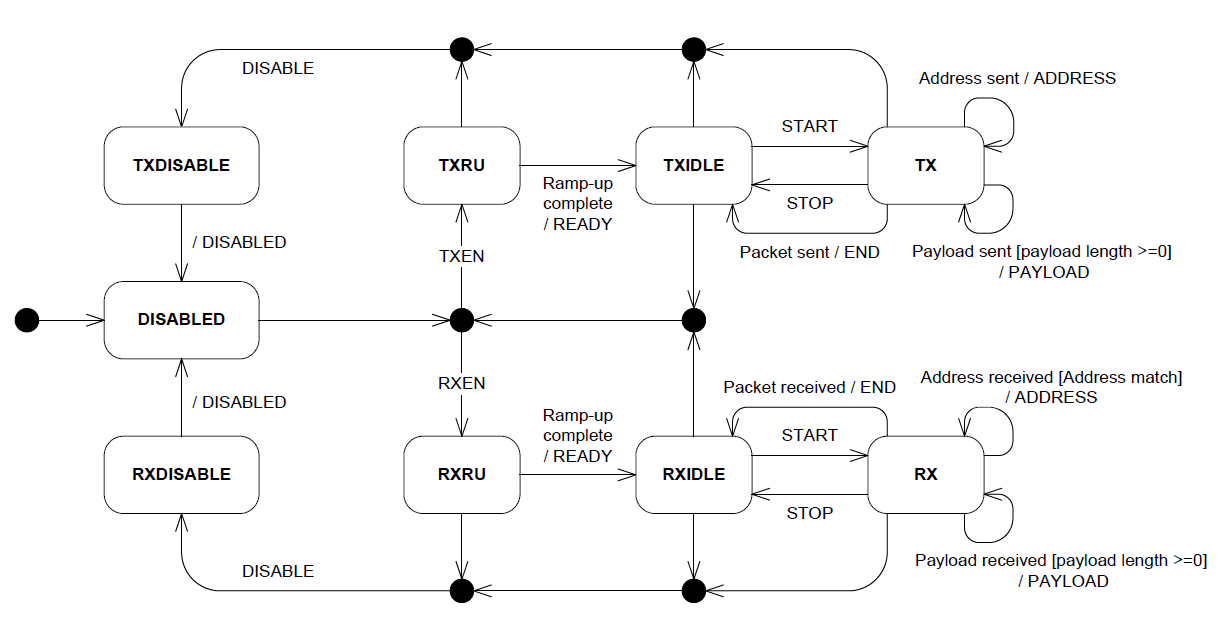
\includegraphics[width=400pt]{txrx_states}
\centering
\caption{Diagramma degli stati per il dispositivo Radio che comprende le fasi di Invio e Ricezione.}
\label{txrx_states}
\end{figure}

Avviando la task per la ricezione, tramite il comando 
\begin{minted}[fontsize=\footnotesize,breaklines]{c}
NRF_RADIO-> TASKS_RXEN = 1U; 
\end{minted}
si imposta la Radio nello stato RXRU. Successivamente controllando quando il valore del campo EVENTS\_ READY assume il valore 1, si può sapere se il dispositivo Radio è pronto per la ricezione. Avviando poi il task di Start, la radio andrà nello stato RX. Per conoscere quando un pacchetto è stato completamente ricevuto si deve controllare il valore del campo EVENTS\_ END, se è 1 un pacchetto è stato ricevuto.
Il controllo della correttezza del CRC non avviene in automatico ma va verificato controllando il valore del campo CRCSTATUS, se 1 il CRC calcolato corrisponde a quello inviato con il pacchetto e quindi il pacchetto è stato ricevuto senza errori. Ad ogni ricezione la Radio va disabilitata, per poter tornare allo stato iniziale e ricevere il pacchetto successivo.

Ogni pacchetto ricevuto deve essere inviato alla UART; vanno prima aggiunti i caratteri di controllo e il separatore (Marker) dei pacchetti, ed è necessario controllare se il pacchetto catturato contenga il valore 0xE0, in quel caso va aggiunto un ulteriore Byte al pacchetto in successione a quest'ultimo per evitare che venga riconosciuto erroneamente come un Marker. Va quindi calcolata la lunghezza totale del pacchetto così modificato e inserita nei Byte 1 e 2  cosicché il ricevitore, dall'altro lato della comunicazione seriale, sappia quanto è lungo il pacchetto e riesca ad identificare eventuali errori di trasmissione se si vede arrivare un Marker prima che il pacchetto inviato abbia raggiunto la lunghezza dichiarata.
Sul dispositivo Nano2 esiste una funzione di libreria che permette di inviare un singolo Byte alla UART e conoscerne il momento dell'effettivo invio, così da evitare di terminare l'invio precedente e sovrascriverlo con uno nuovo; la funzione va quindi chiamata con un while che ne attende il completamento dell'invio:

\begin{minted}[fontsize=\footnotesize,breaklines]{text}
while(NRF_SUCCESS != app_uart_put(ch)); 
\end{minted}

\subsection{Ricevitore seriale}
Dall'altro lato della comunicazione UART è stato usato un PC con sistema operativo Linux, nello specifico Ubuntu 17.04, che ha il vantaggio di supportare nativamente le trasmissioni in seriale andando a creare uno speciale file, /dev/ttyACM0 , in cui si trovano scritti tutti i dati ricevuti da seriale. Leggendo il file è si ottengono i pacchetti inviati dal Nano2 che vanno poi elaborati, visualizzati a video e salvati su un file per analisi future.
\'E stato creato un programma, scritto in linguaggio C, che permette di svolgere le funzioni sopra citate; essendo la trasmissione asincrona, esso deve innanzitutto aspettare la ricezione di un Marker singolo, che indica l'inizio di un nuovo pacchetto, andare a leggere i 2 Byte successivi e ottenerne la lunghezza, e mediante un ciclo for, andare a leggere tutti i Byte successivi e presentarli a video, salvandoli anche sempre su un file secondario.
Per svolgere queste funzioni è stata progettata una macchina a stati, replicata poi in linguaggio C mediante il costrutto \emph{Switch(state)}, mostrata in figura \ref{uart_machine_state}.

\begin{figure}[H]
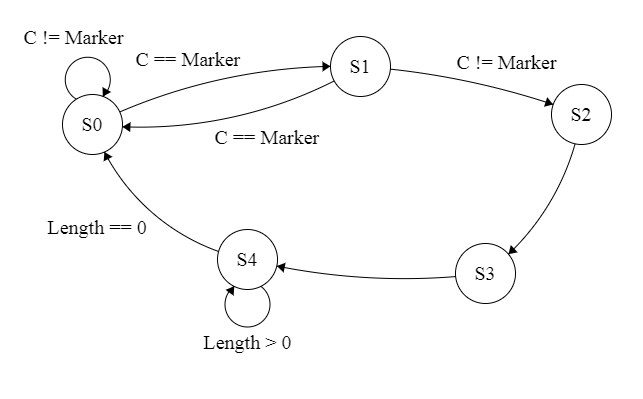
\includegraphics[width=400pt]{uart_machine_state}
\centering
\caption{Diagramma della macchina a stati implementata in C per ricevere i dati dalla UART.}
\label{uart_machine_state}
\end{figure}

Lo stato 0 analizza tutti i Byte scritti nel file alla ricerca del Marker singolo, se lo trova avanza nello stato 1. Qui se il Byte successivo è anch'esso un Marker, siamo di fronte ad un falso Marker e si deve tornare nello stato 0 ad aspettare un nuovo Maker, se invece il Byte è diverso allora esso è il byte più significativo della lunghezza, che va letto e salvato in una variabile; si passa automaticamente nello stato 2 dove si legge il restante Byte della lunghezza avendo quindi ad ora la lunghezza del pacchetto da stampare. Nello stato 3 si va a leggere il 4° Byte del pacchetto che indica in che canale è stato catturato e si va a scrivere subito l'informazione; si procede direttamente nello stato 4 dove si andranno a leggere e stampare tutti i restanti Byte del pacchetto, andando di volta in volta a decrementare la variabile length finché non assume il valore 0 ed il pacchetto è stato interamente letto e si torna quindi nello stato iniziale 0.

\subsubsection{Seguire una connessione}
Per catturare i pacchetti di tipo Advertise è sufficiente sintonizzarsi su un canale di Advertise (37, 38 o 39) e tramite l'AA e CRCInit noti per tutti i pacchetti di Advertise si ricevono tutte le comunicazioni dei dispositivi che vogliono farsi individuare nell'area adiacente allo Sniffer. Un qualsiasi dispositivo che invia pacchetti di Advertise lo fa sempre sui i 3 canali dedicati; uno sniffer quindi è sufficiente che si metta in ascolto su uno dei 3 per poter catturare tutti i pacchetti di questo tipo. Il procedimento si fa più complicato quando si deve andare ad intercettare il pacchetto di CONNECT\_ REQ, perchè viene inviato soltanto su 1 dei 3 canali, ed inviato una sola volta.
Per ovviare a questo problema ci sono varie soluzioni; la prima, la più elementare ma che si adatta a tutti i possibili scenari, è fissarsi su un canale e forzare il dispositivo target a riconnettersi più volte finché non manderà la CONNECT\_ REQ sul canale in cui siamo in ascolto. Una seconda soluzione è creare un dispositivo di Advertising a piacimento che faccia Advertise solo sul canale in cui siamo in ascolto; il dispositivo che vorrà connettersi con quest'ultimo dovrà obbligatoriamente, seguendo le specifiche del protocollo BLE, inviare la sua richiesta di connessione sul canale in cui siamo in ascolto. L'ultima soluzione, la più efficacie ma anche più complessa e costosa, è avere 3 sniffer, uno per ogni canale di Advertise che forniscono una sicurezza del 100\% di riuscire ad intercettare il pacchetto di CONNECT\_ REQ.
Per seguire successivamente la connessione bisognerà ottenere alcuni valori dal pacchetto di connessione catturato; l'AA contenuto nei Byte [15],[16],[17],[18] CRCInit nei Byte [19],[20],[21] e il valore dell'Hop Increment contenuto negli ultimi 5 bit del pacchetto. Successivamente si deve impostare la struttura NRF\_ RADIO con i valori estratti dal pacchetto di connessione per catturare unicamente i pacchetti della connessione;
La parte più complessa è gestire il cambio di canale con le tempistiche esatte per riuscire a ricevere tutti i pacchetti della connessione. Dalle specifiche Low Energy è noto che l'intervallo di connessione, ovvero il tempo in cui la connessione avviene entro un determinato canale, è fisso e deciso in fase di connessione. Questo intervallo inizia nello stesso istante in cui il dispositivo Central invia il primo pacchetto; l'istante viene definito come Anchor Point, ovvero punto di ancoraggio per la connessione.
Non esiste però una funzione di libreria della Nordic che permette di ottenere questo istante, ci si può però basare sull'istante in cui viene ricevuto l'indirizzo, che si può conoscere tramite funzioni di libreria,  e togliere il tempo che è trascorso per ottenere l'istante iniziale in cui il pacchetto è stato trasmesso, dato che l'indirizzo viene trasmesso sempre un numero fissato di Byte dopo l'inizio del pacchetto e la velocità di trasmissione è nota e costante.
Dopo aver fissato l'anchor point, utilizzando la gestione del channel hopping descritta nel capitolo \ref{freqHopping}, è possibile seguire la connessione ed ottenerne tutti i pacchetti.

\subsection{Problematiche riscontrate}
Il progetto dello Sniffer che riuscisse anche a seguire una connessione tra due dispositivi target ha presentato non pochi scogli; la prima grossa problematica è nata sulla cattura della CONNECT\_ REQ. Questo pacchetto, fondamentale per poter ascoltare una connessione, nelle prime versioni dello Sniffer non riusciva ad essere mai catturato. Indipendentemente dai canale di Advertise in cui si era in ascolto o dal numero di tentativi di connessione che di provavano o dalla potenza trasmissiva usata, il pacchetto di connessione non compariva mai nell'elenco dei pacchetti catturati.
La soluzione di questo problema è stata trovata analizzando con il dispositivo USRP i tempi che intercorrevano tra i vari pacchetti di Advertise e la richiesta di connessione; si è notato che essa avveniva con un tempo minore del millisecondo dopo un pacchetto di Advertise. Il problema è stato individuato nella lentezza della trasmissione del dispositivo UART che impegnava per più di un millisecondo la CPU e che quindi non riusciva a riattivare in tempo il dispositivo Radio per ricevere la CONNECT\_ REQ. Inibendo l'invio dei pacchetti di Advertise catturati, ma inviando solamente quello relativo all'evento di connessione, è stata immediata la sua cattura.

Successivamente alla riuscita della cattura del pacchetto di connessione si è quindi provato a impostarci su un canale di connessione, in modo fisso, per vedere se si riusciva nella cattura di un pacchetto.
Partendo dal presupposto che i valori dell'AA e del CRCInit che il Nano2 catturava non erano da usare nell'ordine in cui li inseriva nel pacchetto catturato ed usando come similitudine il comportamento che utilizzava per altri campi del pacchetto, si è pensato che il loro valore reale fosse una specularità Byte a Byte del valore reperibile dal pacchetto. Seppur con svariati tentativi di connessione e inibendo anche la verifica del CRC, concentrandosi quindi unicamente sulla correttezza dell'Access Address, non si è riuscito a catturare nessun pacchetto nei canali data. \'E stato grazie ad un uso verboso dei log che si è individuato il problema: il dispositivo poco dopo l'avvio andava in crash. Questo comportava il riavvio dello stesso con la conseguenza che tutti i dati estratti dal pacchetto di connessione andavano sempre persi e quindi era impossibile catturare un qualsiasi pacchetto nei canali data. Solo risolvendo la causa del crash, ovvero un Null Pointer sulla struttura UART, è stato possibile catturare il primo pacchetto nei canali data.

\subsection{Sviluppi futuri}
Con lo svolgimento di questo lavoro di Tesi si sono create le basi per la creazione di un dispositivo di Relay, un sistema in grado di catturare tutti i pacchetti inviati da un certo dispositivo e replicarli ad una distanza di molto maggiore della portata trasmissiva del protocollo BLE; questo sistema può venire usato per implementare l'attacco Man in the Middle, ovvero un attacco informatico in cui un dispositivo attaccante ritrasmette e/o altera la comunicazione tra due parti che credono di comunicare direttamente tra di loro; nell'ambito Bluetooth questo attacco permette di far credere a 2 dispositivi lontani  di essere a breve distanza e di comunicare. 
La riuscita di questo tipo di attacco permette di svelare le vulnerabilità di tutti quei sistemi che utilizzano la vicinanza tra 2 dispositivi Bluetooth come metodo di accesso a dispositivi protetti da un sistema di sblocco, normalmente con password.
Ad oggi sono sempre di più le applicazioni che utilizzano un sistema keyless per permettere l'accesso ai soli autorizzati, basti pensare ad una serratura della porta principale di un'abitazione, che viene automaticamente sbloccata quando qualcuno in possesso della chiave si trova nelle strette vicinanze della porta e apre semplicemente la maniglia; con un relay di questo tipo un potenziale malintenzionato potrebbe intercettare il proprietario della casa mentre è ad esempio al supermercato, avvicinarlo con un dispositivo di ascolto mentre un suo complice si trova davanti alla sua porta di casa e con il dispositivo di ritrasmissione aprire facilmente la porta di casa.
L'utilizzo di un dispositivo a basso costo rende più facile ed economica la creazione di un relay bluetooth, che può essere reperito ed utilizzato da un numero maggiore di attaccanti; come citato nelle premesse è molto importante che il protocollo trasmissivo BLE sia sicuro ed adotti misure per impedire che attacchi di questo tipo possano funzionare.

Per la creazione di un relay funzionante deve ancora essere sviluppata la parte di trasmissione dei pacchetti catturati a lunga distanza, attraverso mezzi trasmissivi come la rete cellulare utilizzando il protocollo LTE. Per la creazione del dispositivo che ritrasmette i pacchetti catturati, è già stato creato del codice funzionante che permette la trasmissione di pacchetti completamente personalizzati, utilizzato ampiamente nelle fasi di test dello Sniffer.